Modify \texttt{heat\_trbdf2.m} (see Exercise 9.2) to solve the heat equation for $-1 \le x \le 1$ with step function
initial data as above. Test this routine using $k = 4h$ and estimate the order of accuracy as $k \to 0$ with even $m$.
Why does the TR-BDF2 method work better than Crank-Nicolson?

\begin{solution}\ \\\\
    We let $k = 4h$ (i.e., $\alpha = 4$); the output of \texttt{problem\_3b.m} is given below:
    
    \begin{figure}[h]
        \centering
        \begin{verbatim}
                 h            k          error
            1.0526e-01   4.2105e-01   8.3634e-03
            5.1282e-02   2.0513e-01   1.6774e-03
            4.0816e-02   1.6327e-01   1.0951e-03
            2.5316e-02   1.0127e-01   4.0824e-04
            2.0202e-02   8.0808e-02   2.6897e-04
          
         Least squares fit gives E(h) = 0.868668 * h^2.08217
        \end{verbatim}
        \caption{Output of \texttt{problem\_3b.m}}
    \end{figure}
    
    \begin{figure*}[h]
        \centering
        \begin{subfigure}[b]{0.425\textwidth}
            \centering
            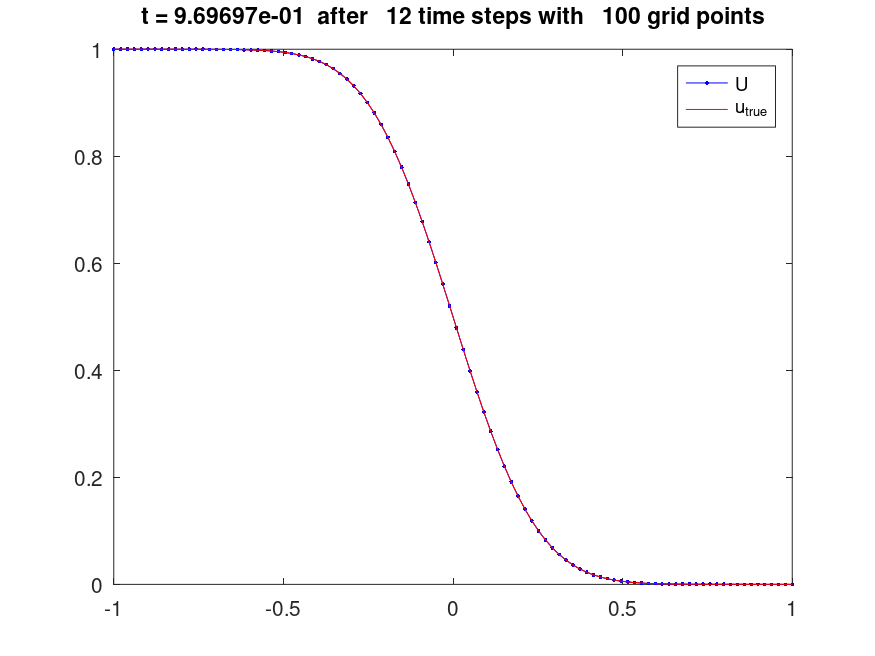
\includegraphics[width=\textwidth]{problem_3b_heatTRBDF2_t-12.png}
            \caption{TR-BDF2 method for $m = 98$ at $t = 1$}
        \end{subfigure}
        \hfill
        \begin{subfigure}[b]{0.4\textwidth}
            \centering
            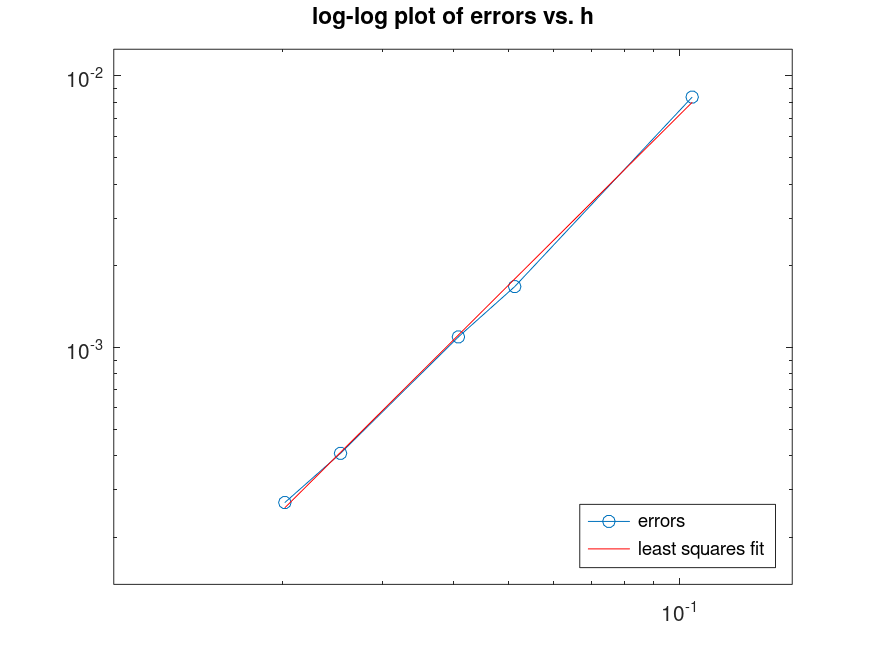
\includegraphics[width=\textwidth]{problem_3b_heatTRBDF2_error.png}
            \caption{TR-BDF2 error}
        \end{subfigure}
        \caption[]{TR-BDF2 solution}
    \end{figure*}

    The least squares fit from above corresponds to $h$ versus error, and because \linebreak
    $\Delta t = k = h = \Delta x$, we observe that our order of accuracy is $\mathcal{O}\left(h^2 + k^2\right)$. In
    particular, the Crank-Nicolson method is derived by way of appplying the trapezoidal rule to the MOL discretization.
    In the case of this problem, our initial solution is discontinuous and encodes an extremely rapid transient at
    $x = 0$. Since the trapezoidal rule is A-stable but \textit{not} L-stable, we expect it to perform poorly for this
    problem. The TR-BDF2 method, in contrast, is L-stable (and of course therefore A-stable as well), and so does not
    suffer from the same instability issue observed with the Crank-Nicolson method.
    \ \\
\end{solution}